\section{SDN în contextul reţelelor actuale}

Chiar dacă nu este o tehnologie ajunsă la maturitate în toate aspectele unei rețele, paradigma \gls{sdn} este deja folosită în rețele de producție de anumite tipuri. Autorii din \cite{alvizu2017comprehensive} evidenţiază faptul că evoluția \gls{sdn} este susţinută de către trei mari porţiuni ale industriei rețelisticii: furnizorii serviciilor de tip \textit{cloud} (care utilizează mari centre de date), furnizorii de servicii de telecomunicaţii și întreprinderile, așa cum se poate observa și în Figura \ref{fig:sdn_network_deployments}. 

\begin{figure}[h]
	\centering
	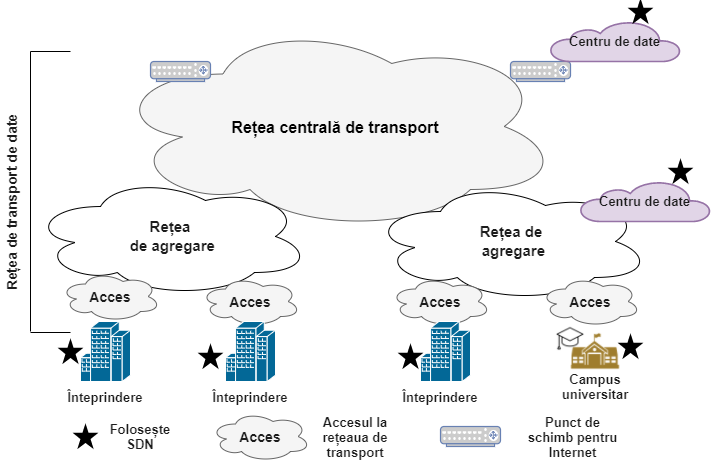
\includegraphics[width=1\textwidth]{sdn_network_deployments}
	\caption{Implementarea SDN în contextul rețelelor actuale~\cite{alvizu2017comprehensive}}
	\label{fig:sdn_network_deployments}
\end{figure}

Astfel, \gls{sdn} este implementat deja cu succes în rețelele unor campusuri universitare (Universitatea Stanford, de exemplu, dat fiind faptul că această paradigmă își are originile acolo), în mari centre de date sau în întreprinderi. În cazul rețelelor de transport, încă se duc activităţi de standardizare care să permită operatorilor rețelelor de telecomunicaţii să implementeze această tehnologie în cel mai scurt timp, beneficiind astfel de avantajele pe care aceasta le oferă (cel mai important, din punctul lor de vedere, fiind reducerea costurilor).

Această secţiune va prezenta în continuare utilizarea \gls{sdn} la momentul actual, în mai multe contexte: în rețelele din marile centre de date, în rețelele de tip hibrid, care combină rețelele tradiționale cu \gls{sdn} sau prin studii de caz, implementări sau experimente efectuate pe teren (în rețele de producție).

\subsection{SDN în centrele de date}

Centrele de date reprezintă grupări de calculatoare cu putere mare de procesare și capacitate mare de stocare. Această idee nu este una nouă, fiind prezentă de câteva decenii, însă, în timp, au evoluat caracteristicile calculatoarelor, precum și numărul lor într-un centru de date. În zilele noastre acestea au ajuns sa conţină mii sau chiar zeci de mii de mașini fizice (servere) \cite{goransson2016software}.

Creșterea numărului de servere și a puterii de stocare, combinate cu creșterea vitezei și a lărgimii de bandă din rețea a dus la necesitatea de a stoca din ce în ce mai multă informație în centre de date tot mai mari. În mod natural, acest lucru va însemna combinarea centrelor de date pentru a forma altele mai mari. Pe lângă acest aspect, se pune foarte mare accent în ultimul timp pe tehnologii de virtualizare, care permit unui server rularea mai multor mașini virtuale, pentru diferite aplicații sau servicii ale utilizatorilor.

A fost creat astfel un mediu dinamic, atât în cadrul centrelor de date, cât și între acestea. După cum este prezentat și în \cite{onf_openflow_backbone2012}, operații precum prevenirea sau recuperarea în caz de dezastru, sau echilibrarea încărcării severelor au nevoie de o creștere a traficului între centrele de date, lucru ce duce la o administrare mai complexă a acelei rețele.

Centrele de date sunt folosite și în cazul oferirii de servicii de virtualizare de servere. Operaţiunile într-un astfel de mediu implică lucrul cu mașini virtuale și, de cele mai multe ori, necesitatea migrării acestora între diferite mașini sau centre de date. Asta înseamnă că diferite aplicații sau servicii trebuie să aibă o imagine proprie asupra rețelei dintre servere, care este doar o vedere la nivel logic, în comparaţie cu rețeaua fizică existentă. Așa cum este prezentat și în \cite{nadeau2013sdn}, crearea de astfel de rețele logice se poate face si fără \gls{sdn}, prin metode folosite și în rețelele tradiționale, cum ar fi cu ajutorul unor \gls{vlan}-uri. Însă, în cazul centrelor de date foarte mari, acestea pot fi insuficiente. Cum ele pot fi exprimate într-un pachet Ethernet doar prin 12 biţi, numărul maxim de rețele virtuale este 4096. Apare astfel nevoia unor alte metode, care sunt însă mai complex de configurat.

O metodă pentru crearea de rețele logice care să fie prezentate unor aplicații sau servicii este chiar folosirea tehnologiei \gls{sdn}, făcând abstracţie de rețeaua fizică. În \cite{onf_openflow_backbone2012, onf_sdn_datacenter2013, liu2014sdn, munoz2015integrated} se prezintă diferite metode care pot fi aplicate în astfel de cazuri, sau care chiar au fost demonstrate.

Soluția \gls{sdn} a fost chiar aplicată în rețele de producție. Așa cum se explică în \cite{google_casestudy}, centrele de date ale Google folosesc deja această soluție, cu ajutorul protocolului OpenFlow. Există două laturi ale rețelei de arie largă - \gls{wan} folosită de Google: o parte legată la Internet, care conţine traficul utilizatorilor și o parte internă, care transportă traficul dintre centrele de date. Cele două au caracteristici diferite ale traficului și, implicit, nevoi diferite. În acea rețea internă a fost implementat \gls{sdn}, prin protocolul OpenFlow. Avantajele evidenţiate de Google includ o viziune de ansamblu asupra rețelei, un răspuns mai rapid la erori, timp mai scurt de implementare, actualizări mai rapide ale software-ului rețelei, fără pierdere de trafic sau existența unui mediu de test de mare fidelitate. Chiar dacă în 2012, atunci când a fost implementată această tehnologie în rețea, protocolul OpenFlow era încă la început și nu avea toate facilităţile pe care le oferă astăzi, Google a arătat încă de atunci că tehnologia \gls{sdn} poate fi folosită, aducând foarte multe avantaje, în multe cazuri de utilizare din industria rețelisticii.

\subsection{SDN în rețelele hibride}

Rețelele hibride reprezintă o combinație între rețelele tradiționale și \gls{sdn}, având scopul de a combina avantajele aduse de ambele, cât timp tehnologia \gls{sdn} nu este încă destul de matură și prezintă unele dezavantaje. Un alt motiv pentru apariția acestor rețele hibride este imposibilitatea de a schimba rețelele de producție într-un timp foarte scurt, în același timp asigurând și funcționarea acestora în parametrii agreaţi.

Autorii din \cite{vissicchio2014opportunities} prezintă oportunităţile și provocările aduse de o astfel de abordare. Ei propun patru modele ale rețelelor hibride: (i) rețele hibride bazate pe topologie, (ii) rețele hibride bazate pe servicii, (iii) rețele hibride bazate pe clase și (iv) rețele hibride integrate. Avantajele prezentate de aceste modele hibride sunt flexibilitatea, robusteţea, extensibilitatea, costuri mai mici ale implementării, date de faptul ca nu toată rețeaua este actualizată. Pe de altă parte, această abordare vine și cu dezavantaje, reprezentate de nevoia de a administra paradigme eterogene și garantarea faptului că interacţiunea dintre ele este benefică.

În \cite{hong2016incremental, levin2013toward, canini2016panopticon} se propun sisteme care să permită o implementare incrementală a \gls{sdn} în rețele de tip hibrid pentru rețele ale întreprinderilor și ale furnizorilor de servicii. Autorii evidenţiază faptul că implementarea directă, într-o rețea de producție a acestei noi tehnologii este imposibilă și ar conduce atât la probleme de implementare, cât și la probleme operaționale în rețea. Ei susţin că implementarea \gls{sdn} în puncte cheie ale rețelelor va aduce avantajele acestei tehnologii, fără nevoia de a înlocui toată rețeaua de la început. Pentru a determina aceste puncte cheie, autorii propun un \textit{planificator al implementării}, care să analizeze topologia de rețea, împreună cu informaţiile istorice despre trafic și constrângeri de resurse.

Lucrarea \cite{jin2015telekinesis} prezintă o altă abordare pentru aceste rețele hibride. Autorii propun un echipament de control al rețelei care să poată interacţiona atât cu echipamentele care folosesc un control centralizat, cât și cu cele care au un control distribuit. Controlarea echipamentelor vechi din rețea, care nu suportă protocolul OpenFlow se face chiar cu ajutorul acestuia. Astfel, dacă se vrea alterarea fluxului de date dintr-un echipament vechi, autorii propun folosirea unei extensii a OpenFlow, numită \textit{LegacyFlowMod}, care să instruiască un echipament OpenFlow să trimită un alt pachet special către echipamentul vechi, astfel încât acesta să își schimbe tabela de dirijare.

Autorii din \cite{caria2015divide, caria2016link} susţin de asemenea că o soluție hibridă este mai potrivită. Propun astfel folosirea unor rețele care să combine \gls{sdn} cu protocolul \gls{ospf}, păstrând avantajele date de acest protocol vechi de rutare, care a fost folosit cu succes câteva zeci de ani și, în același timp, aducând și câteva din avantajele propuse de \gls{sdn}.

\subsection{Studii de caz. Implementări. Experimente în rețele de producție}

Există numeroase studii de caz sau experimente în rețele de producție care demonstrează utilitatea \gls{sdn} și faptul că această tehnologie poate fi implementată cu succes în rețelele din zilele noastre.

În \cite{nec2012hospital} se prezintă soluţia implementată în rețeaua spitalului \textit{Kanazawa University}, din Japonia. S-a folosit tehnologia \gls{sdn}, cu ajutorul protocolului OpenFlow pentru a uşura munca de administrare a rețelei spitalului, care devenea din ce în ce mai complexă, pe măsură ce noi echipamente medicale trebuiau adăugate. Rețeaua, fiind operată de personalul spitalului, era vulnerabilă la erorile provocate de greşelile umane. Trebuia asigurată izolarea între anumite departamente ale spitalului, în unele cazuri, astfel că administrarea rețelei devenea greoaie. Cu ajutorul \gls{sdn} a fost creată o soluție în care infrastructura de rețea a devenit mai uşor de administrat, prin aplicații software care rulează deasupra echipamentului de control \gls{sdn}, permiţând departamentelor crearea de rețele virtuale proprii, asigurând în același timp conectivitate între departamente. Astfel, rețeaua spitalului a devenit stabilă și pregătită pentru dezvoltările rapide care apar în industria medicală în zilele noastre.

Lucrarea \cite{bidkar2014field} ilustrează folosirea \gls{sdn} în cadrul unei rețele optice de transport a unui furnizor de servicii prin Ethernet. Autorii au implementat această tehnologie pentru oferirea de servicii în acea infrastructură de rețea. Obiectivele urmărite au fost simplificarea administrării rețelei și furnizarea de trafic, în funcție de serviciul solicitat (de exemplu, lățime de bandă la cerere).

În \cite{kalman2014applicability} se analizează posibilitatea folosirii tehnologiei \gls{sdn} în rețelele Ethernet industriale. Autorul evidenţiază punctele în care această tehnologie s-ar putea aplica în rețelele industriale și avantajele pe care o astfel de implementare le-ar aduce.

Autorii din \cite{kobayashi2014maturing} urmăresc evoluția implementărilor \gls{sdn} pornind de la nivelul unei rețele dintr-un simplu laborator din cadrul Universităţii Stanford și până la rețele de nivel naţional. Cu ajutorul acestor studii se evidenţiază compromisurile care apar în implementarea acestei noi tehnologii în rețele de producție. De exemplu, pentru o simplă rețea a unui campus universitar, un singur server poate susţine tot planul de control al rețelei, incluzând echipamentul de control și diferitele aplicații care rulează acolo pentru administrarea acesteia. Primele cazuri de utilizare demonstrate cu ajutorul \gls{sdn} au fost rutarea pe cea mai scurtă cale de nivel 2, învăţarea adreselor de nivel 2 - \gls{mac}, descoperirea topologiei cu ajutorul \gls{lldp} sau colectarea de statistici de la comutatoarele din rețea. Aceste experimente au subliniat câteva aspecte importante pentru performanţelor rețelelor \gls{sdn}: timpul necesar configurării fluxurilor de date în rețea, numărul de intrări în tabelele de fluxuri ale comutatoarelor. De asemenea, este important ca un comutator să fie hibrid, adică să suporte atât protocolul OpenFlow, cât și pe cele tradiționale. O altă fază a experimentelor conduse de aceşti autori a constat în împărțirea infrastructurii de rețea în mai multe rețele logice destinate diferitelor aplicații. 

Toate aceste experimente și studii de caz prezentate au avut la bază protocolul OpenFlow, ducând la evoluția acestuia. Acest lucru nu trebuie să ne ducă însă cu gândul că tehnologia \gls{sdn} înseamnă doar OpenFlow. După cum se va vedea în capitolele următoare, în special în cazul rețelelor de transport de date prin microunde, există și alte protocoale cu ajutorul cărora se pot aduce principiile \gls{sdn} în rețea.
